\chapter{Implementation}

This chapter covers in details the implementation of the features covered within the design chapter and will list in detail the general implementation of a feature including there issues, it will also detail the environments and tools used to create the application and the supporting services behind the application.

\section{Tools used}

In this section the tools used for building the application and backend services will be detailed and there role within the development of the project as a whole.

\subsection*{Sublime Text}

Sublime Text is one of the main tools that was used throughout the development of the project, it is highly regarded as one of the best text editors in the public space due to its flexibility and community support to help it fit the users needs.\\
\\
It has been a crucial tool for developing the middle tier application as all of the code was written in sublime text, this report that you are reading now was exclusively written in Sublime Text and the vast majority of the SQL was also writing within the Sublime Text editor. In image of the text editor can be found in figure \ref{fig:sublime_text_image}.

\begin{figure}[H]
    \centering
    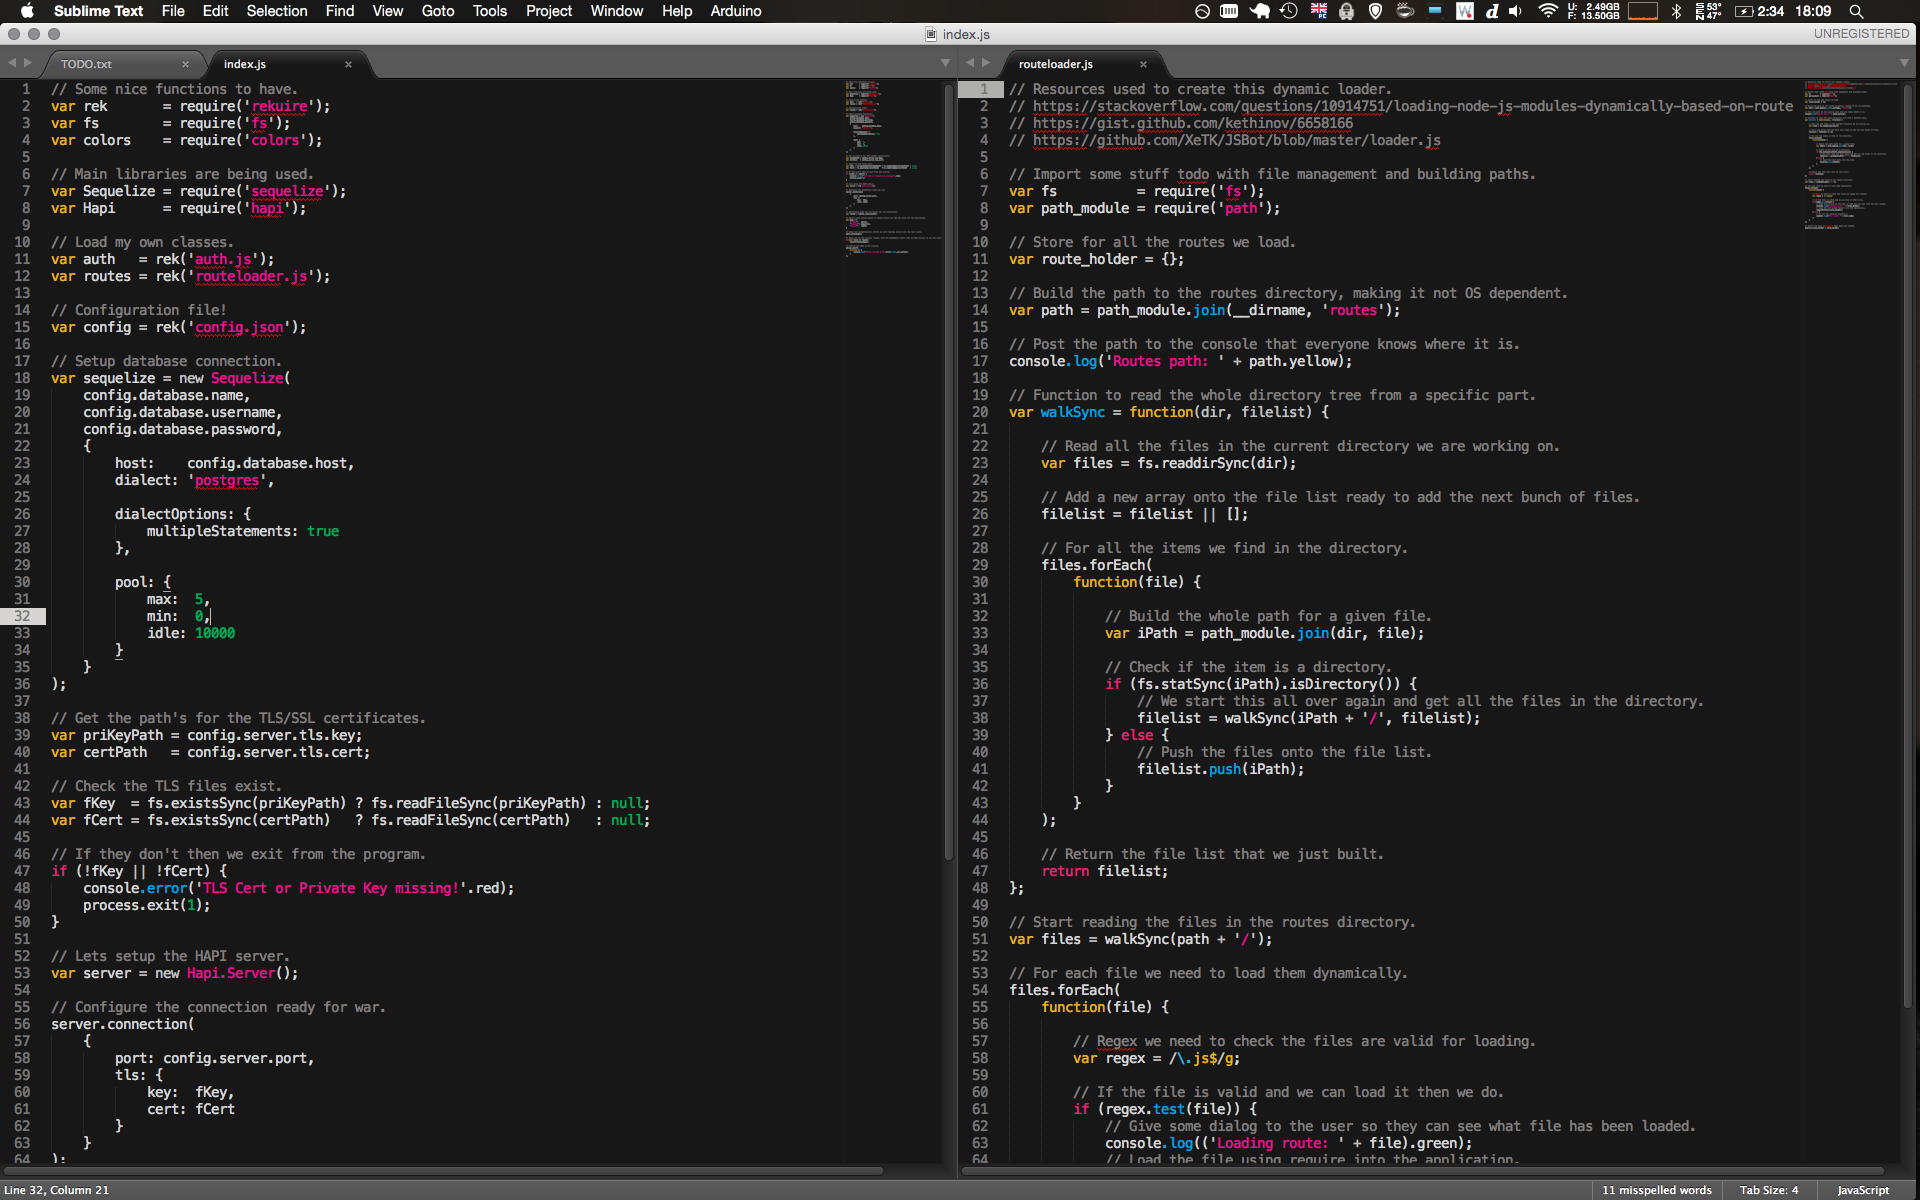
\includegraphics[width=\textwidth]{tools/sublime}
    \caption{Sublime Text 3.0}
    \label{fig:sublime_text_image}
\end{figure} 

\subsection*{Android Studio}

Android Studio has played the most crucial role within the development of the project it has been the integrated development environment of choice for Android development giving all the required features and tools needed to create a fully fledged Android application with the potential of being released into a production environment, it contains all of the testing tools required to do good Android development with a unit testing suite and various UI testing suites.\\
\\
It has close links to the Android SDK so it enables users to use the various Android SDK tools within the Android Studio GUI some of the advanced tools within the Android SDK are covered later in this section. Android Studio offers powerful code completion tools and refactoring tools to speed up the development of the application it also has the ability to error check the code and provide solutions through the development of the project with powerful auto complete tools to build up the stub functions to complete the implementation of imported libraries. An example of the layout and design of Android studio can be found in figure \ref{fig:android_studio_image}.

\begin{figure}[H]
    \centering
    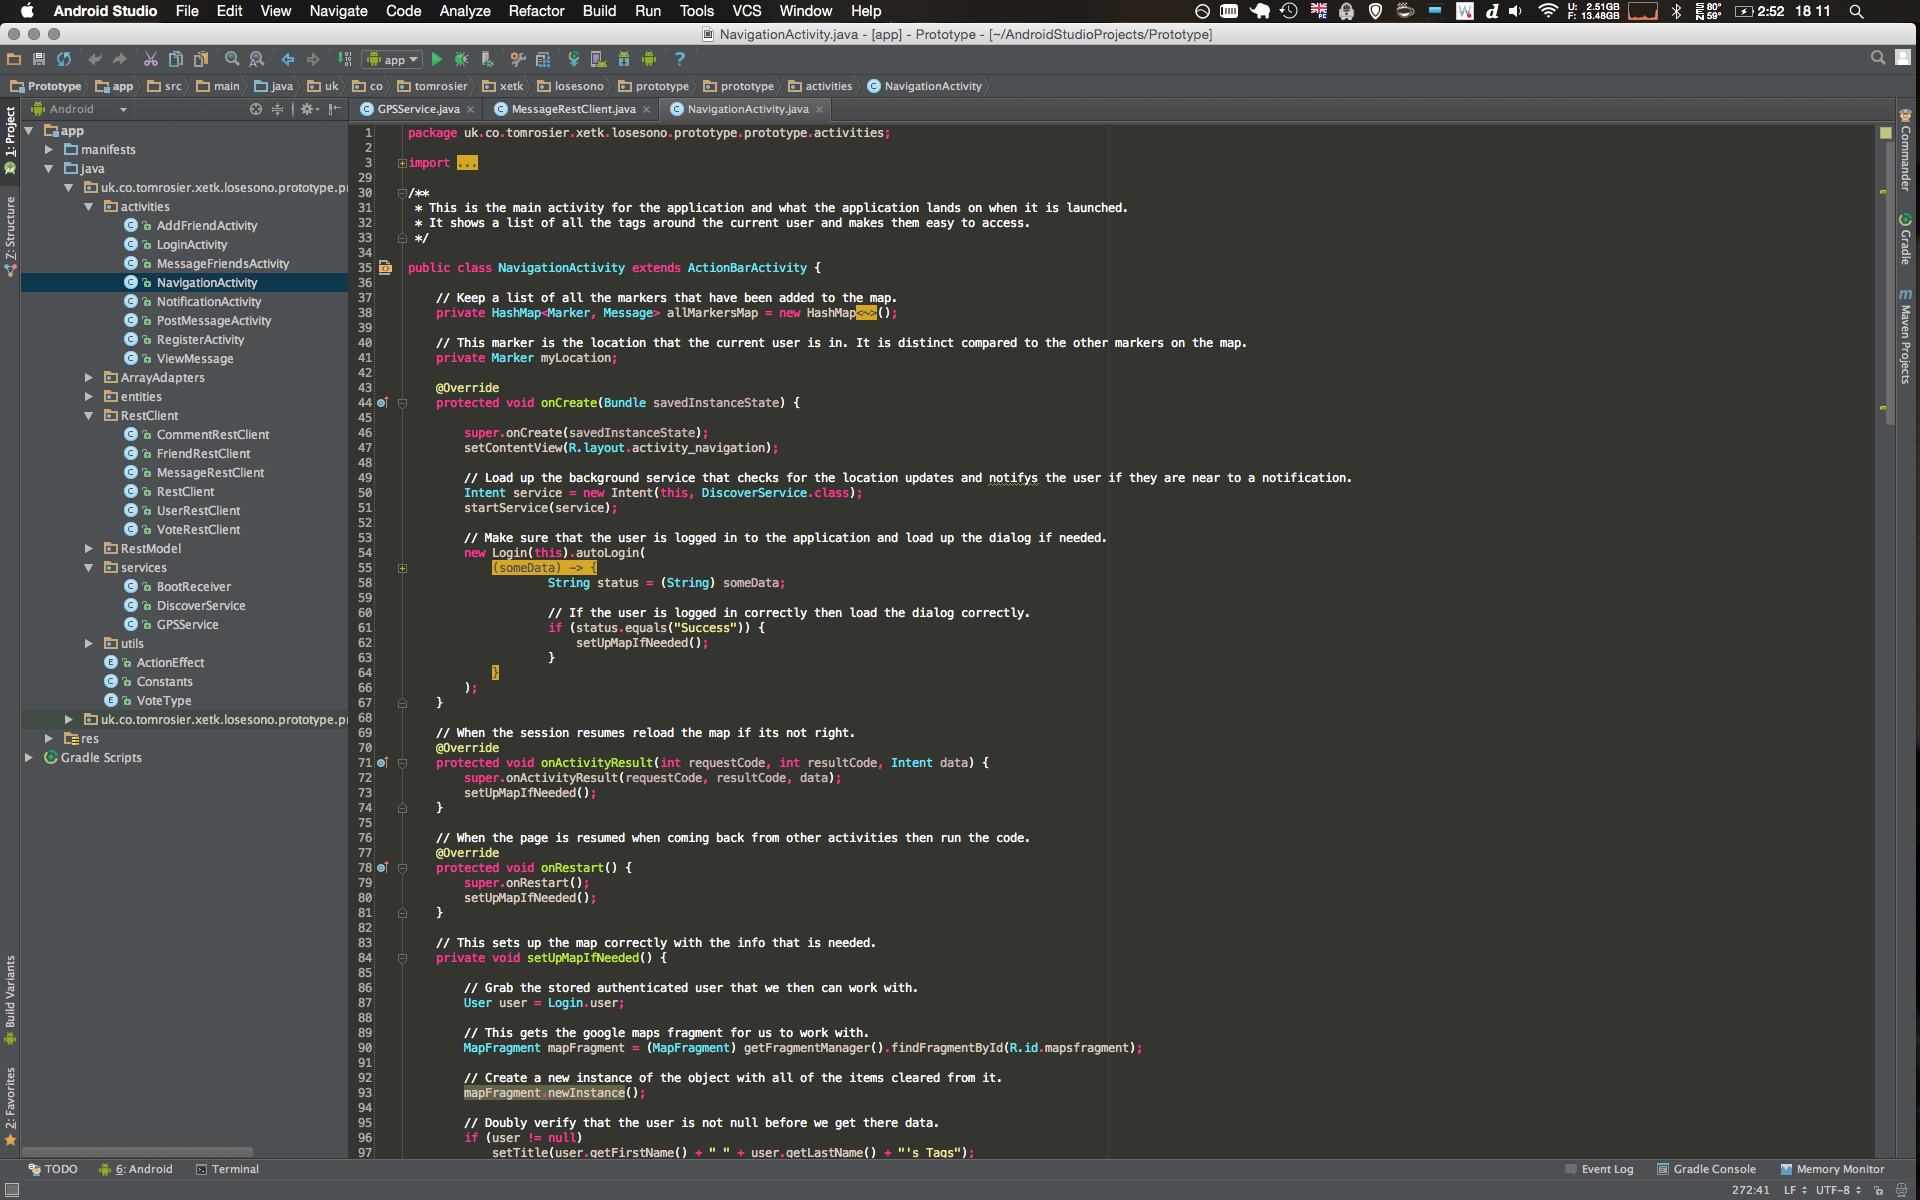
\includegraphics[width=\textwidth]{tools/androidstudio}
    \caption{Android Studio 1.1.0}
    \label{fig:android_studio_image}
\end{figure} 

\subsection*{PGAdmin3}

PGAdmin3 is a tool for remotely accessing Postgres database and allowing management through a GUI based interface, it allows easy access to viewing data held within the database along with the ability to execute SQL commands directly on the database. The tool was mostly used as a verifier to check that SQL executed within the terminal had run correctly and had created the tables and constraints that were needed for the application to work correctly. Small note this crashes a lot on a Apple Mac, An example of the execution of PGAdmin3 can be found in figure \ref{fig:pg_admin_image}.

\begin{figure}[H]
    \centering
    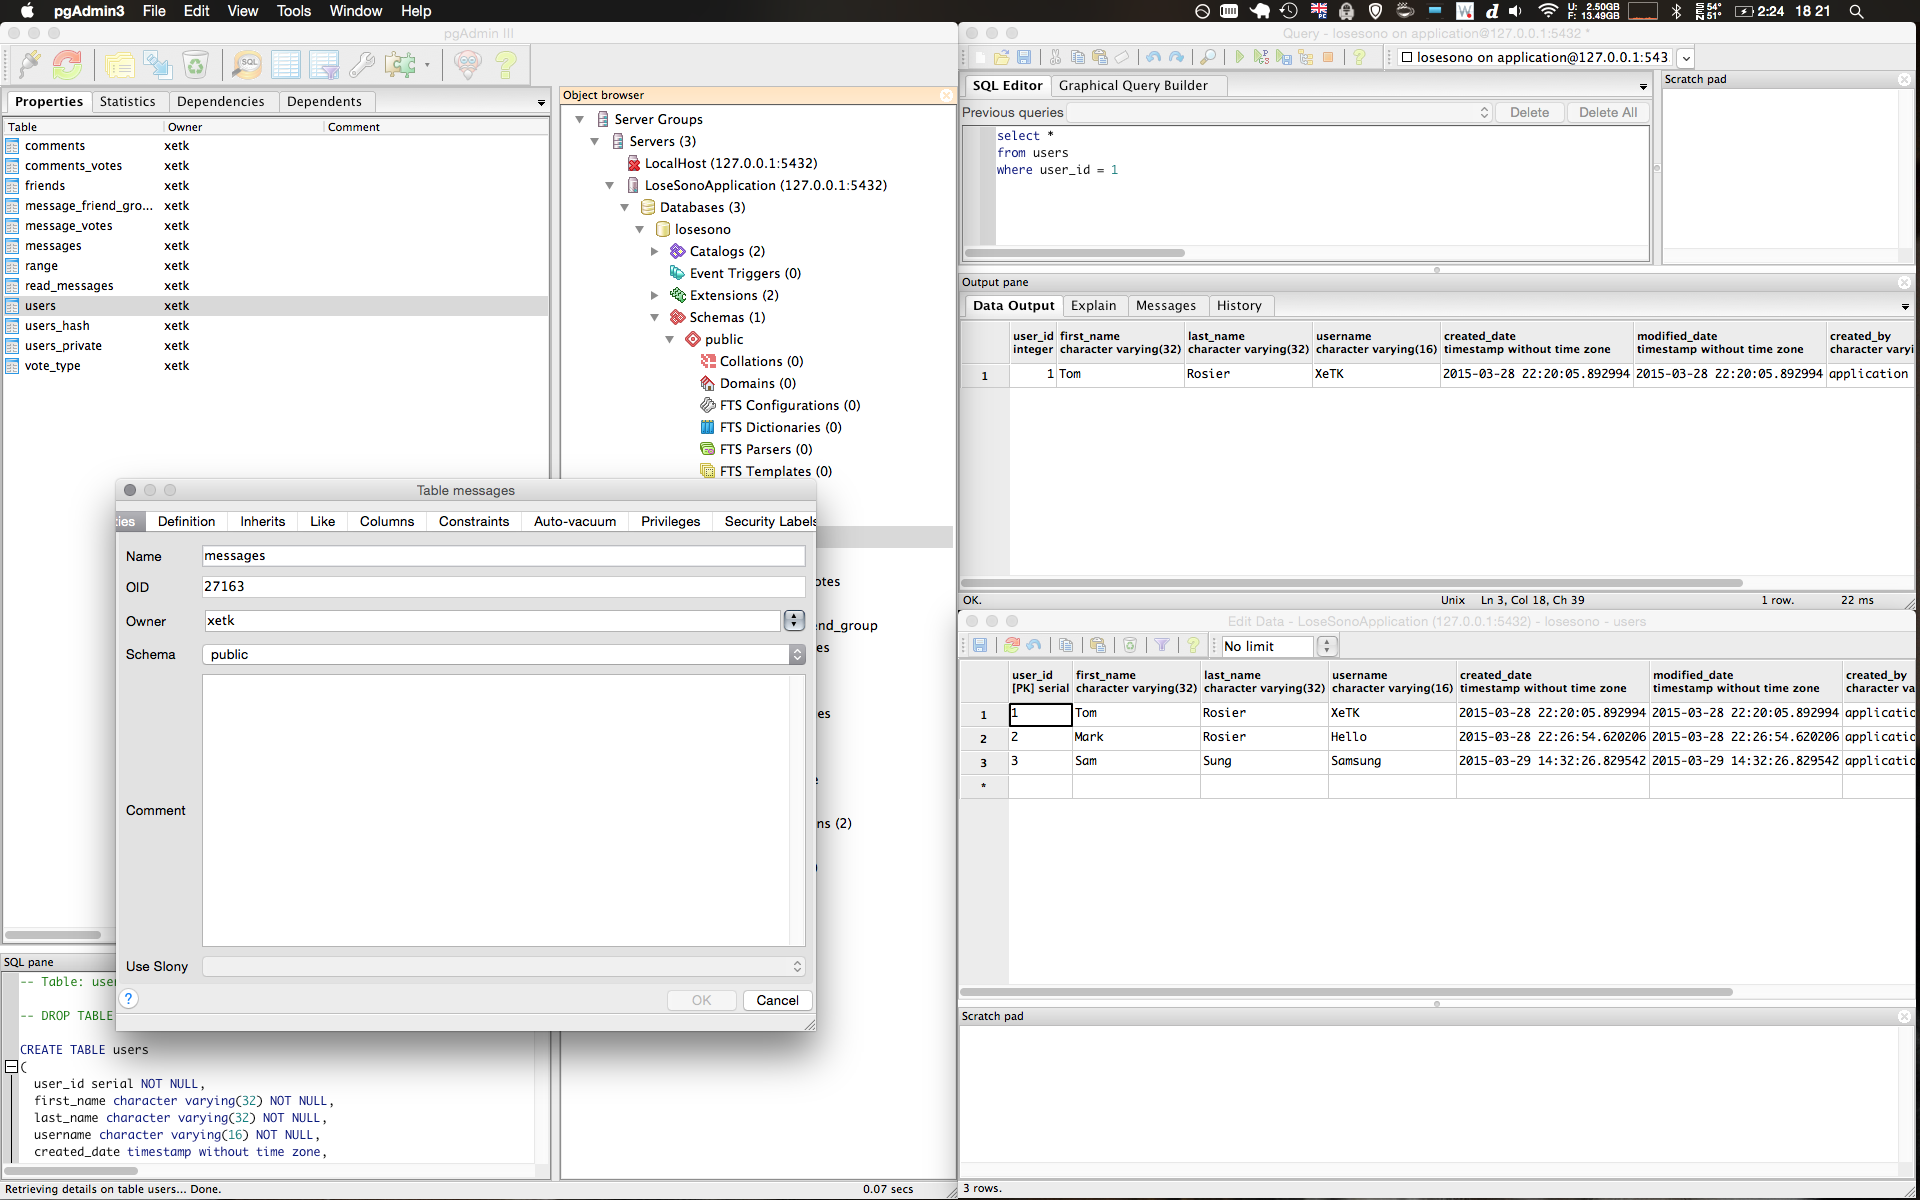
\includegraphics[width=\textwidth]{tools/pgadmin}
    \caption{PGAdmin3 1.20.0}
    \label{fig:pg_admin_image}
\end{figure} 

\subsection*{PGSQL command line}

The PostgreSQL command line tool was used in conjunction with PGAdmin3 to do all the SQL related work needed for the project, the PostgeSQL command line allows direct command execution within the SQL engine so is perfect for debugging issues within the database along with creating the SQL statements to extract the data needed to get the functional requirements of the application working correctly.\\
\\
PostgreSQL its self is fairly difficult to install correctly and there were many issues with getting it to install correctly and work as intended, the command line package manager for Apple Mac Homebrew PostgeSQL's package is completely broken and caused massive headaches at the start of the project theses issues were resolved by installing the official DMG package provided by Postgres.app \cite{jemt:postgresapp:2015:online}.

\begin{figure}[H]
    \centering
    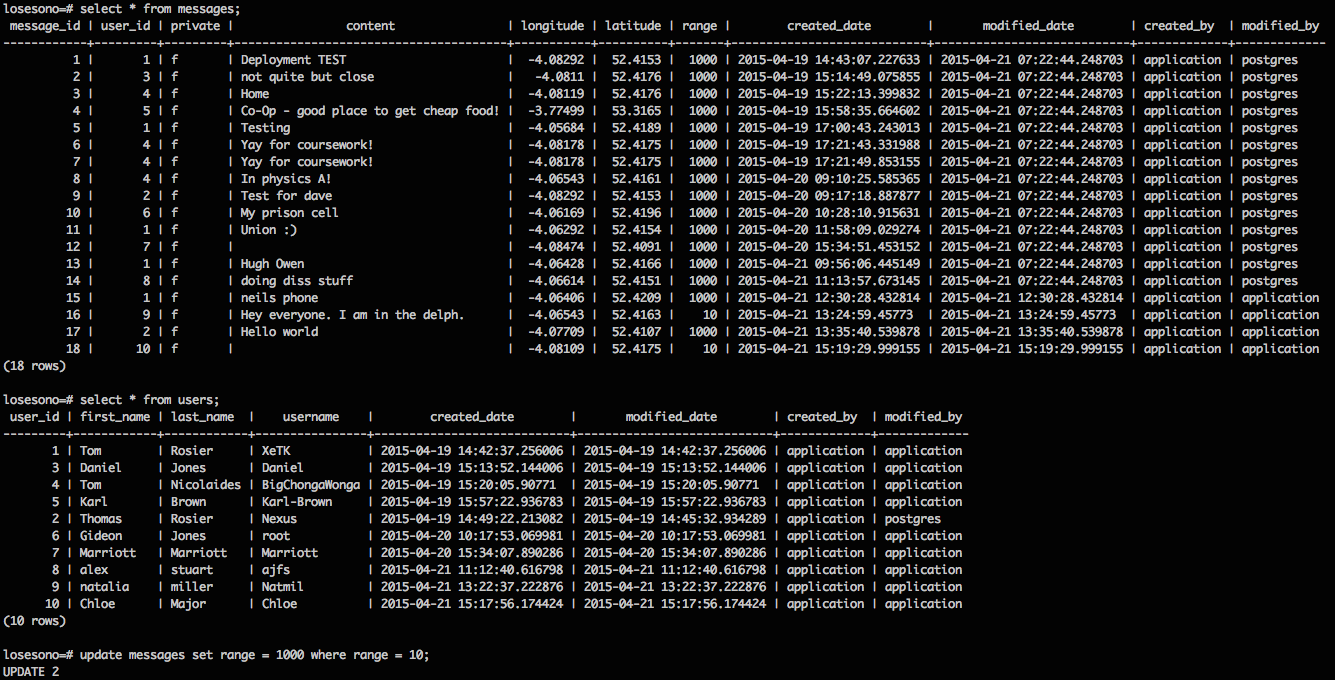
\includegraphics[width=\textwidth]{tools/pgsqlcommandline}
    \caption{PG SQL Command line 9.3.6}
    \label{fig:pg_sql_image}
\end{figure} 

\subsection*{Postman}

Postman was an essential tool for debugging the RESTful interfaces provided by the applications, it enables the emulation of HTTP POST and GET requests enabling the ability to attach the parameters needed when completing a POST request and making sure the interface is working correctly without the need to implementing it fully into the application. It was often used to check if the RESTful interface was working correctly before implementing the corresponding code within the Android side of the application, Postman its self has a few issues, if a request would fail for what ever reason the application would get stuck in the sending request stage and would require closing the tab and re opening. An image of Postman at work can be found in figure \ref{fig:postman_image}.

\begin{figure}[H]
    \centering
    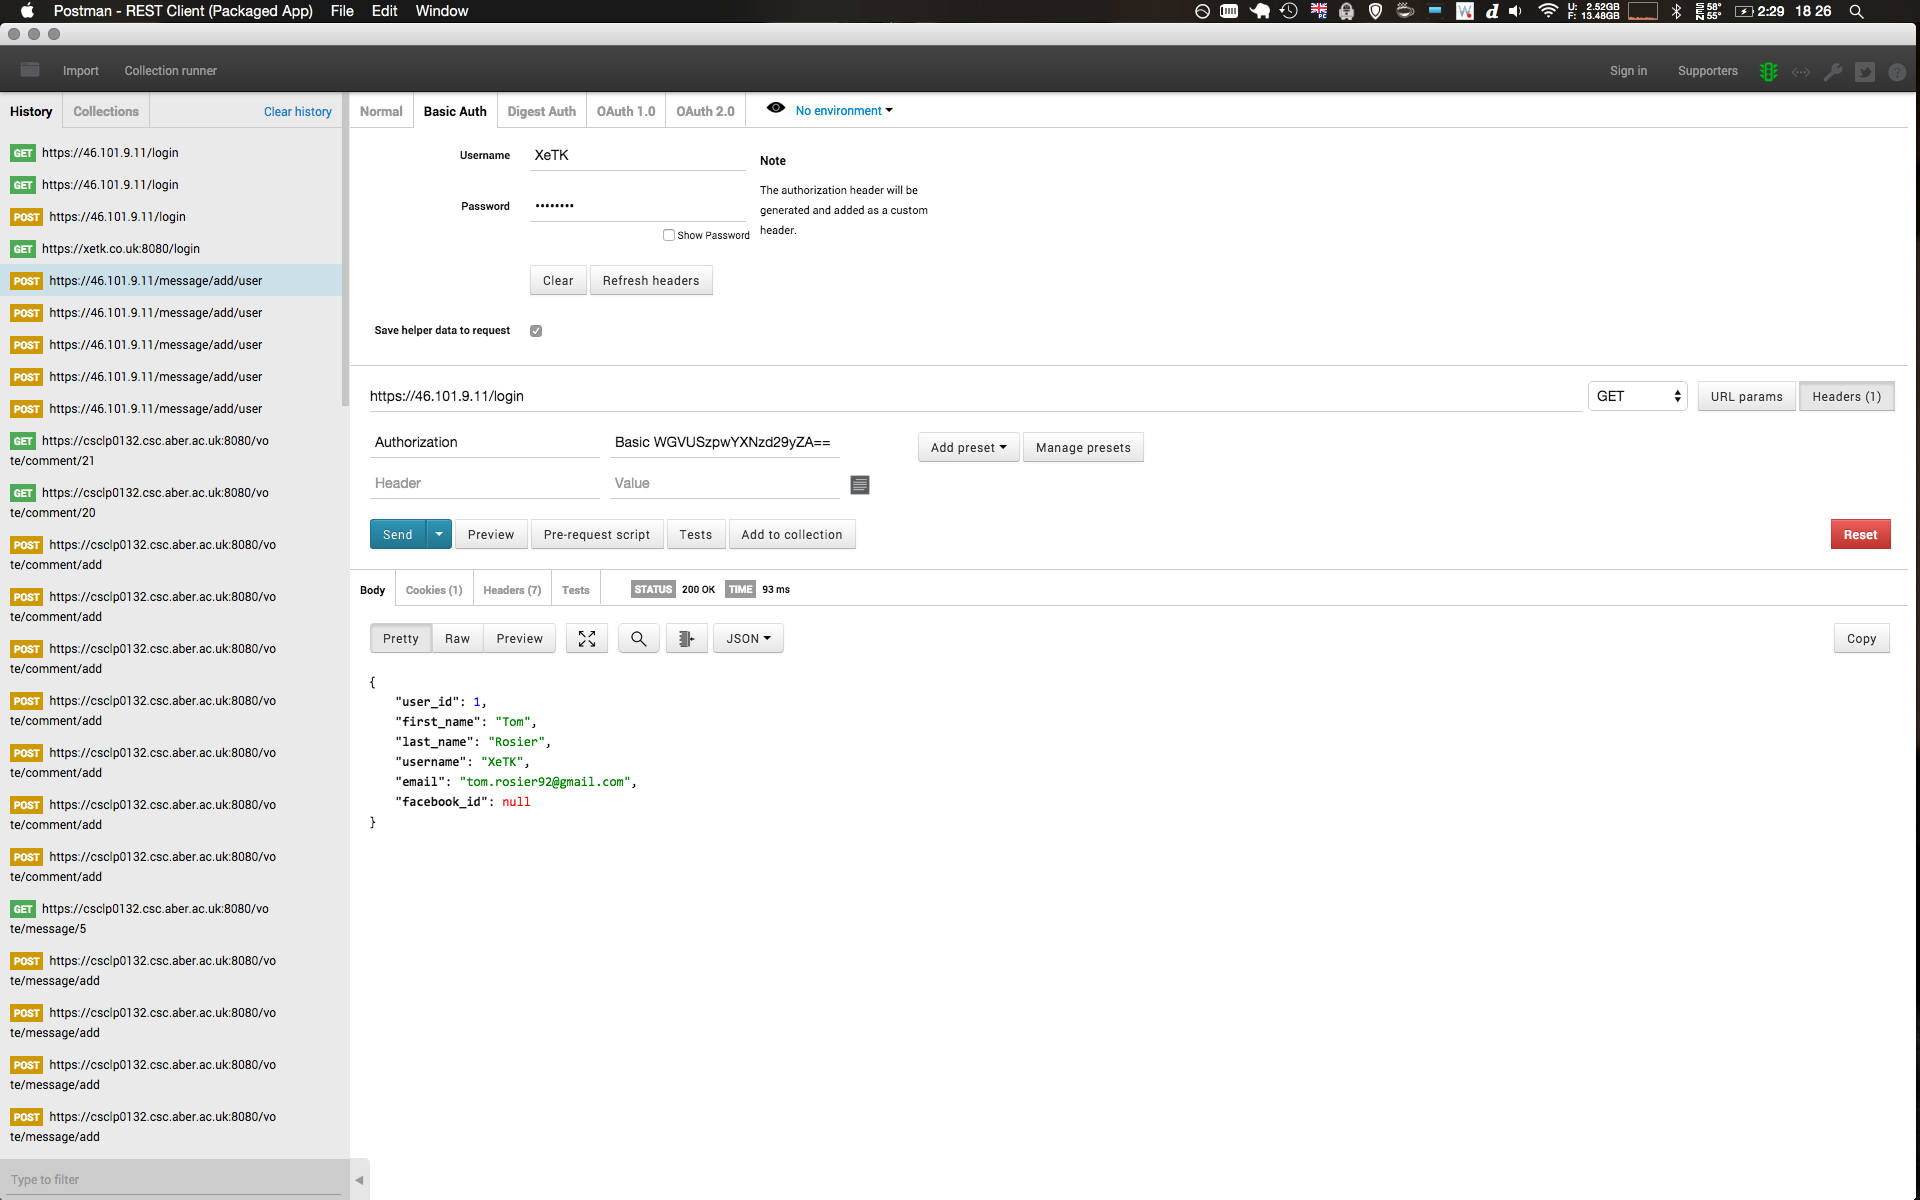
\includegraphics[width=\textwidth]{tools/postman}
    \caption{Postman 2.0.19}
    \label{fig:postman_image}
\end{figure} 

\subsection*{Web browsers}

A web browser is an essential tool in any software related tool in the modern world, It was primary used for researching the project as a whole but it was also used for debugging the backend API as it can carry out HTTP requests, accept cookies and deal with HTTP authentication. They were often used to complement Postman when it could not quite carry out the required action that was needed.\\
\\
The two main browsers used to test the application were Opera And Google Chrome, Opera being my main browser so Chrome was used as a backup when needed. Images of the two main browsers that were used can be found in figures \ref{fig:opera_image} and \ref{fig:chrome_image}.

\begin{figure}[H]
    \centering
    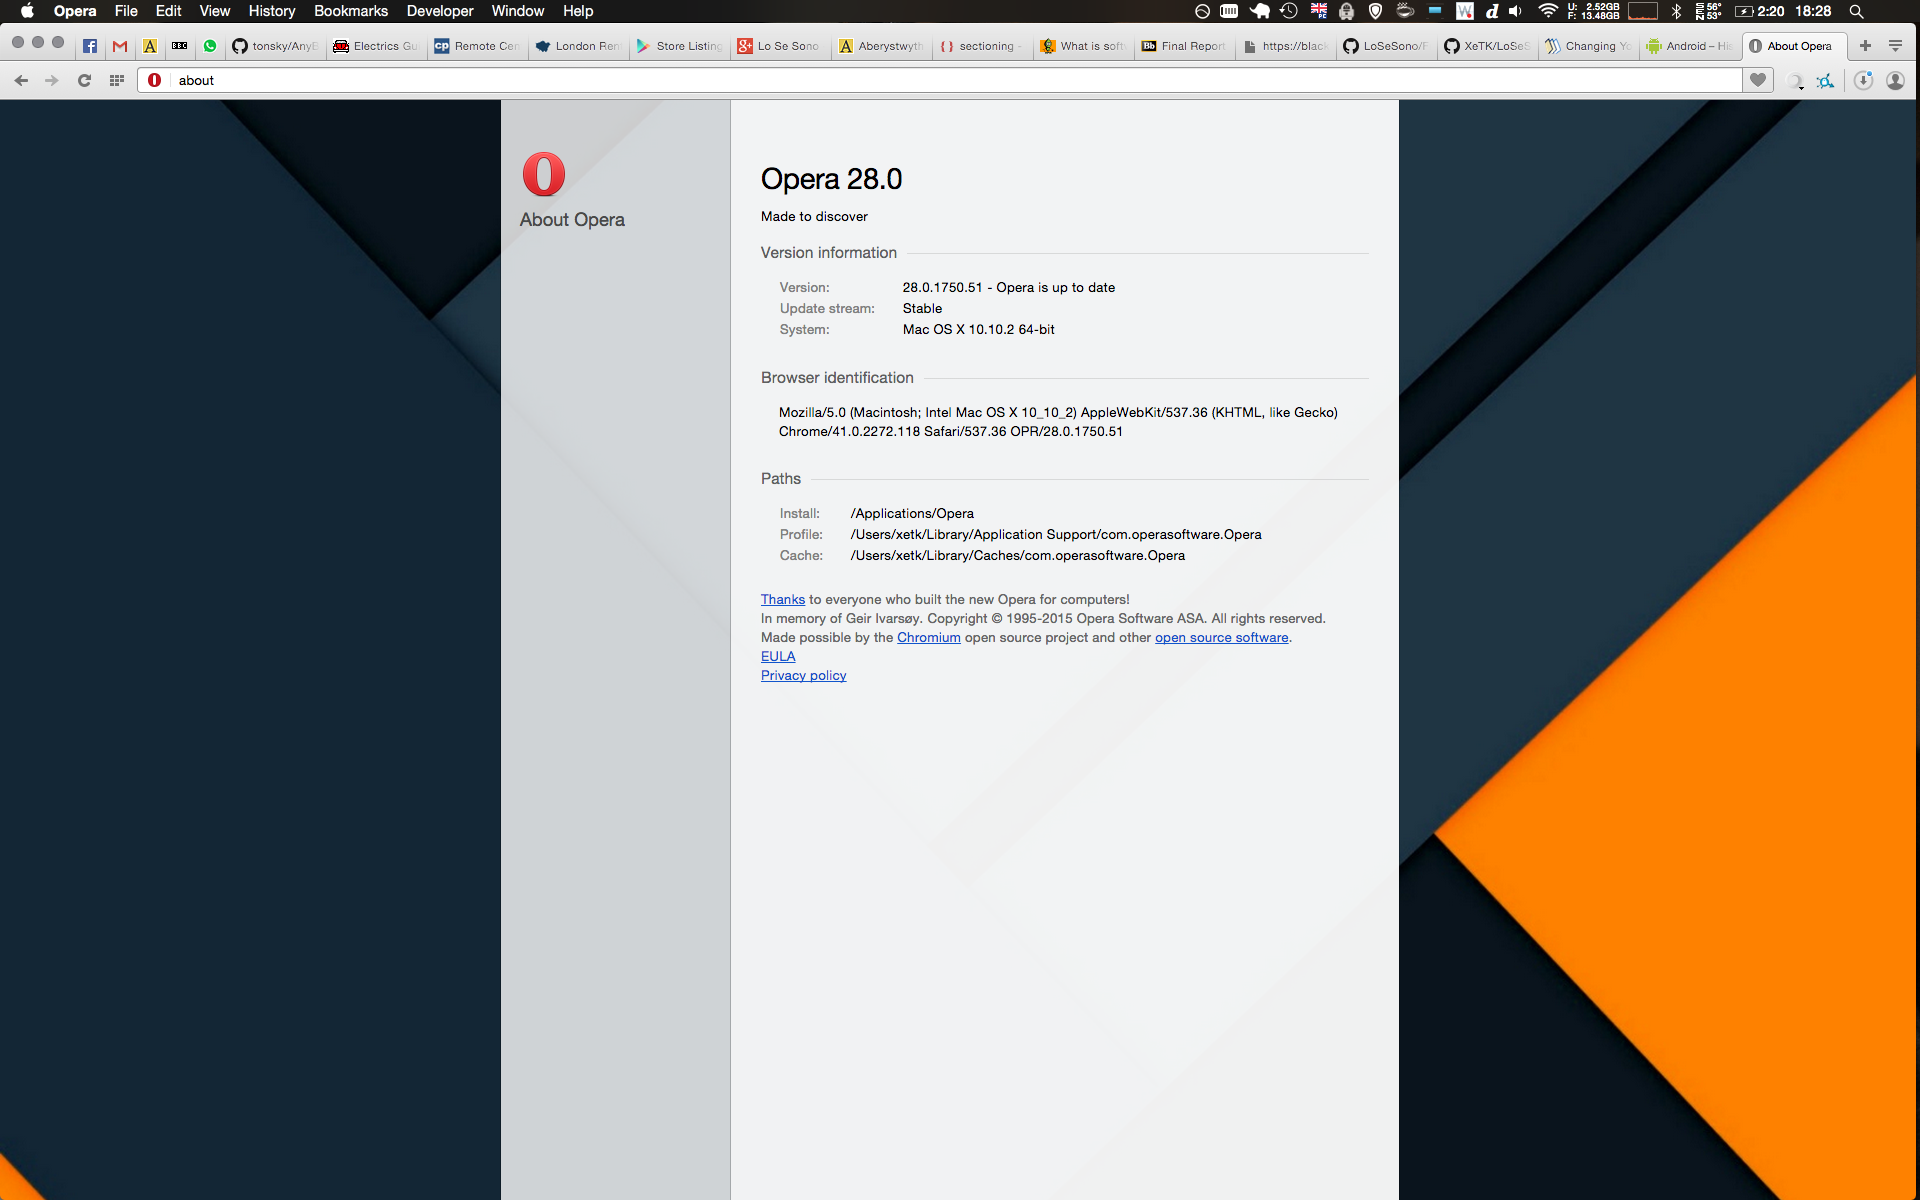
\includegraphics[width=\textwidth]{tools/opera}
    \caption{Opera 28.0}
    \label{fig:opera_image}
\end{figure} 

\begin{figure}[H]
    \centering
    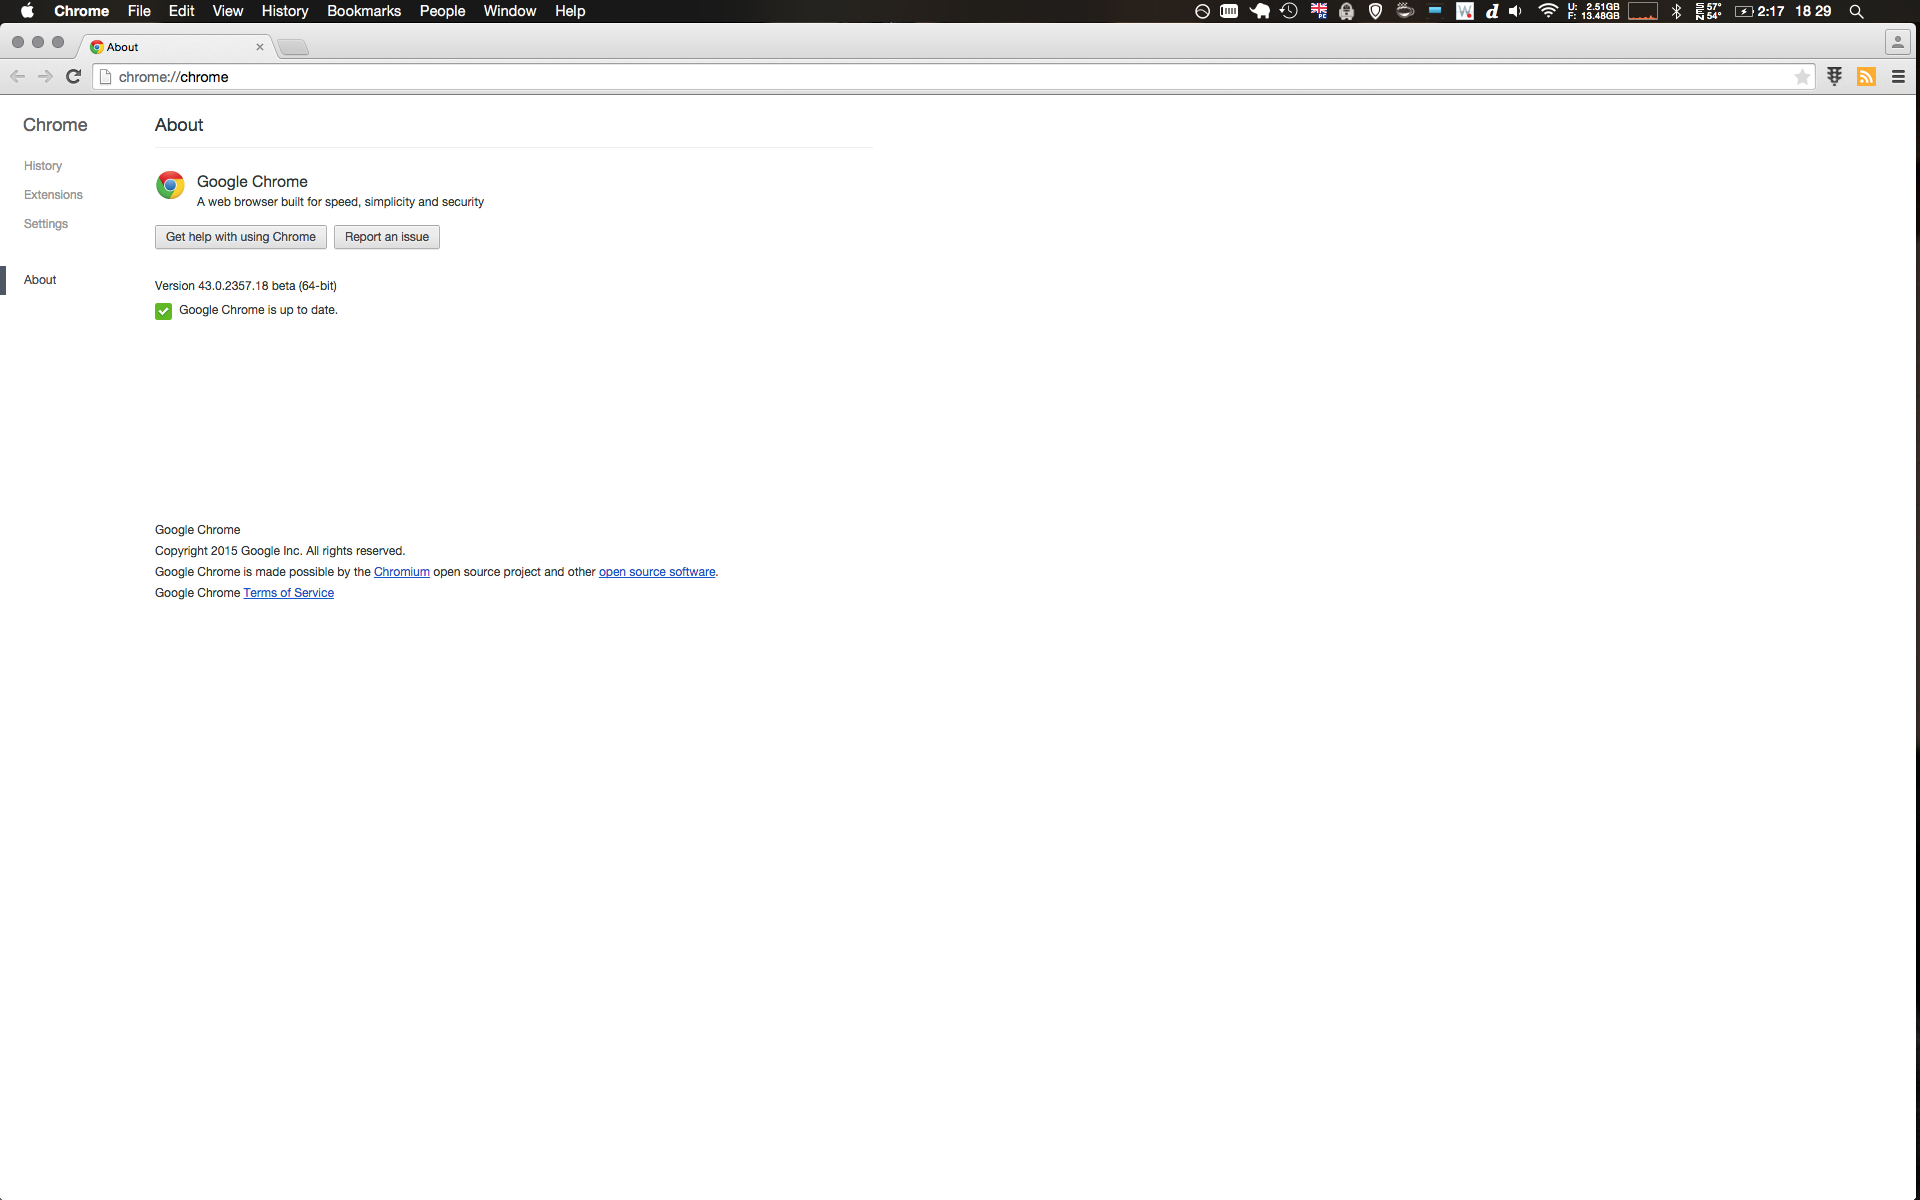
\includegraphics[width=\textwidth]{tools/chrome}
    \caption{Chrome 43.0}
    \label{fig:chrome_image}
\end{figure} 

\subsection*{Android SDK Tools}

Throughout the development of the project there was a need to use the full Android Software Development Kit for testing and debugging the application in the given environment it will be run. The SDK provides all of the build tools needed to create and compile the packages needed to install the application on the device along with submit it to the Google Play Store.\\
\\
The first and possible most used tool throughout the development of the application is the Android Emulator, the tool emulates the Android platform on the development machine to provide an environment to test code without the need of a physical device this can be useful when the developer only has a limited selection of devices to test the application on as the emulator gives the ability to scale to different screen sizes and resolutions to help with debugging on different devices. In figure \ref{fig:android_emulator} shows the emulator at work running the application in a test mode.

\begin{figure}[H]
    \centering
    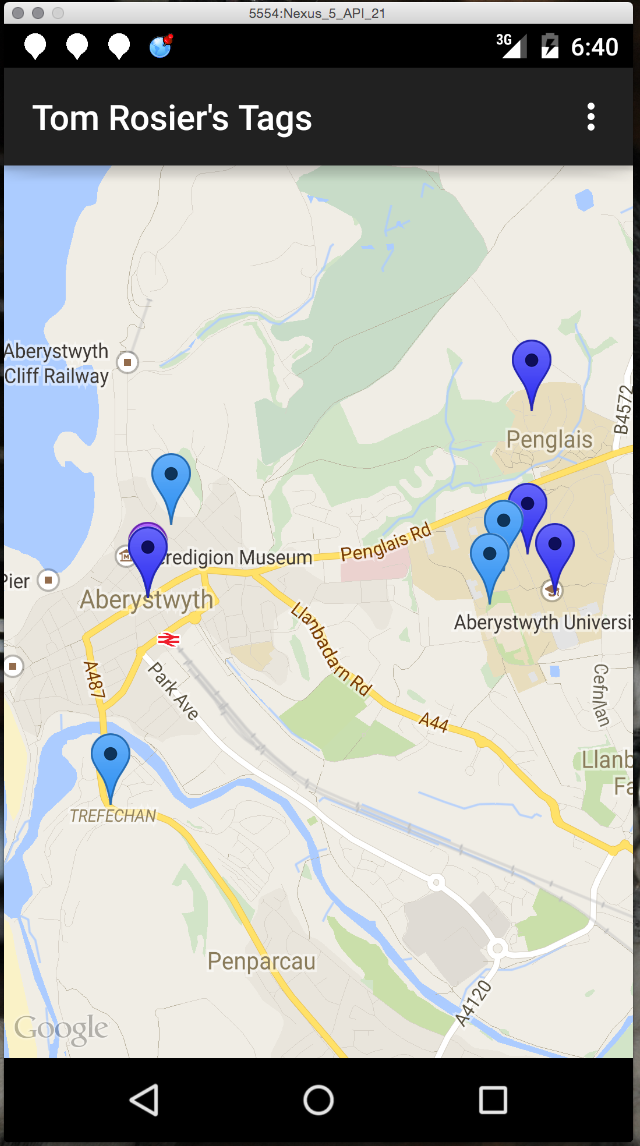
\includegraphics[width=0.5\textwidth]{tools/androidemulator}
    \caption{Android Emulator SDK 22}
    \label{fig:android_emulator}
\end{figure} 

\noindent
Another equally important tool that was used extensively during the development of the project was the command line application Android Development Bridge(ADB). ADB is used to interface with Android based devices and provides many features that allow interfacing and connecting to the device, it is crucial for debugging applications along with working with the Operating System directly. It has been extensively used through this project to repair damaged and broken phones to bring them back to a state where they can be used to help with development.

\begin{figure}[H]
    \centering
    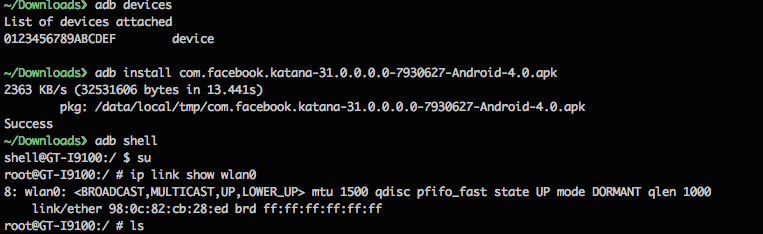
\includegraphics[width=0.75\textwidth]{tools/adb}
    \caption{Android Development Bridge}
    \label{fig:adb_image}
\end{figure} 

\noindent
The SDK updater played a very minor in the project but it allows easy and quick way to update the SDK and build tools within the Android development suite to the latest versions to enable development for newer devices as they come to market.

\begin{figure}[H]
    \centering
    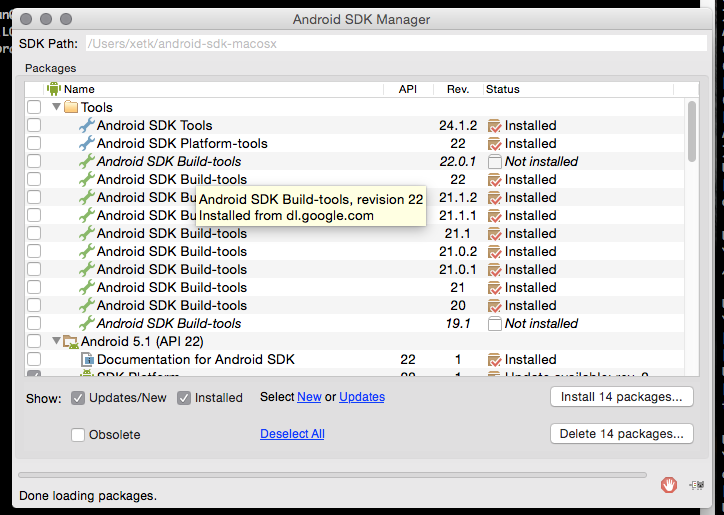
\includegraphics[width=0.75\textwidth]{tools/sdkupdator}
    \caption{Android SDK Updater}
    \label{fig:sdk_updator}
\end{figure} 

\subsection*{Git Hub}

Throughout the project the version control system GIT has been used to ensure that the source code for the project has been reliably backed up and provide the ability to check in versions of the code to return to a prior point if needed.\\
\\
The use of the service GitHub as a on-line repository to keep the code easily accessible and backed up throughout the project along using some of the extra functionality by using a 3rd party to store and look after the source code. In future it will enable people to contribute to the project and do there own tweaks and improvements to ensure that the project becomes a fully fledged and vibrant application. The standard GitHub page layout can be found in figure \ref{fig:git_hub_repos_image}.

\begin{figure}[H]
    \centering
    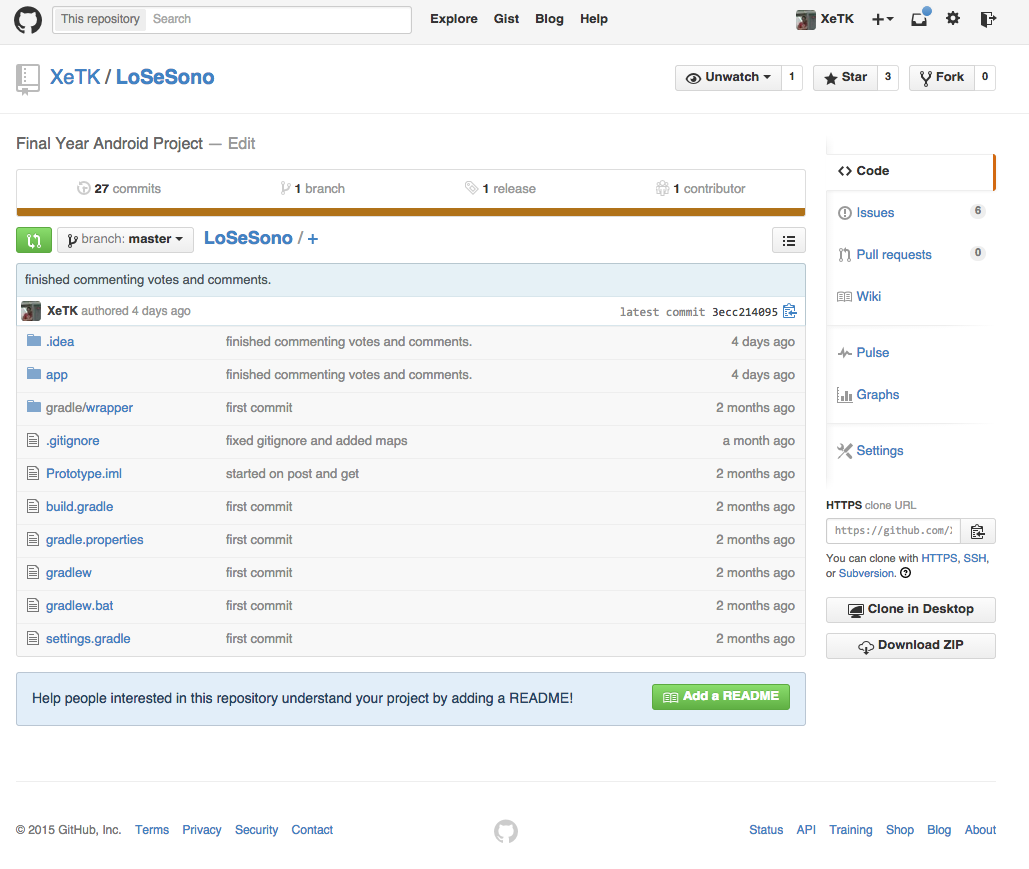
\includegraphics[width=\textwidth]{tools/github}
    \caption{Git Hub git repositories}
    \label{fig:git_hub_repos_image}
\end{figure} 

\noindent
GitHub provides a issue tracker so that users can leave issues and bug reports for the developer to fix or improve, it has been integral throughout the project to keep track of any issues that have been raised within the development of the application.\\
\\
They have been marked as fixed or left ready to be fixed in the future development of the application and gives a traceable history of any issues within the application. The UI for the issue tracker can be found in figure \ref{fig:gh_issue_tracker_image}.

\begin{figure}[H]
    \centering
    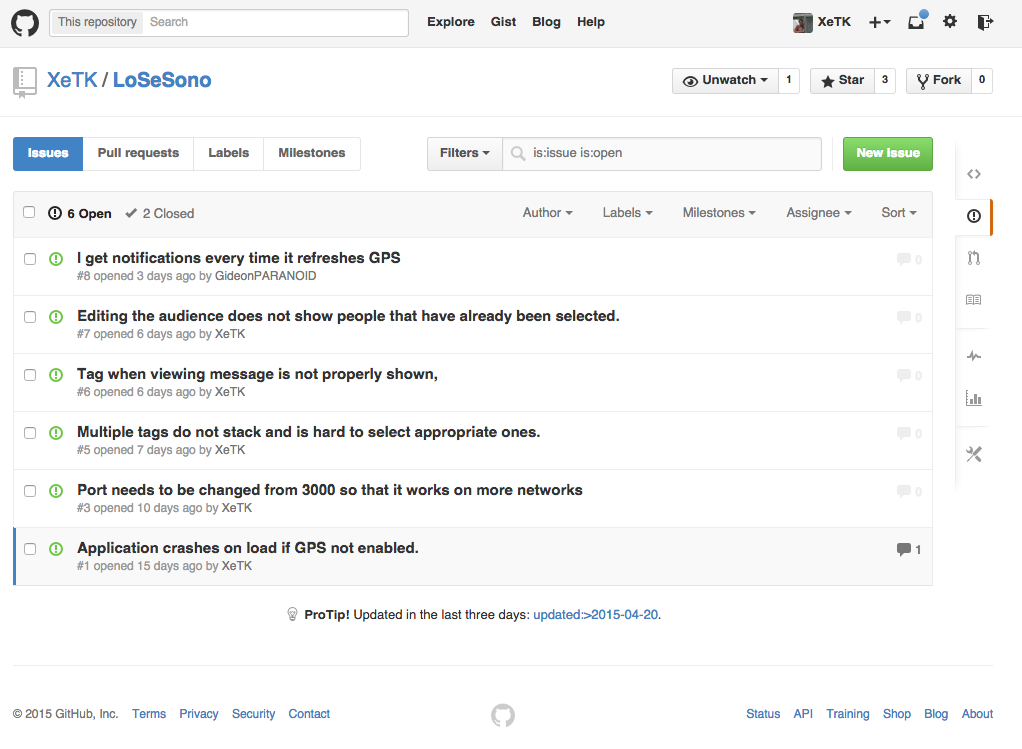
\includegraphics[width=\textwidth]{tools/githubissues}
    \caption{Github issue tracker}
    \label{fig:gh_issue_tracker_image}
\end{figure} 

\section{Android application}

\subsection{Development Hardware}

\subsection{Environment}

\subsection{Features}


\subsubsection*{Login}

\paragraph*{Implementation}

\paragraph*{Issues}


\subsubsection*{Registration}

\paragraph*{Implementation}

\paragraph*{Issues}


\subsubsection*{Adding Friends}

\paragraph*{Implementation}

\paragraph*{Issues}


\subsubsection*{GPS Location}

\paragraph*{Implementation}

\paragraph*{Issues}


\subsubsection*{Maps}

\paragraph*{Implementation}

\paragraph*{Issues}


\subsubsection*{Posting message}

\paragraph*{Implementation}

\paragraph*{Issues}


\subsubsection*{Retrieving messages}

\paragraph*{Implementation}

\paragraph*{Issues}


\subsubsection*{Retrieving notifications}

\paragraph*{Implementation}

\paragraph*{Issues}


\subsubsection*{Comments}

\paragraph*{Implementation}

\paragraph*{Issues}


\subsubsection*{Votes}

\paragraph*{Implementation}

\paragraph*{Issues}



\section{Server side application}

This section covers the overall implementation of the backend services required to get the application working, it will not talk about design this is covered in chapter \ref{ch:design} section \ref{sec:server_side_design}.

\subsection{Environment}

This section covers the environment the application will be run in with the server side. The development environments slightly from the technologies covered in this section, instead of a Linux based machine running the application the development system used is a Apple Mac, this should not create any issues as the technologies chosen are highly portable and work on many different operating systems.

\subsubsection{Debian based Linux}

For running the server side services it was decided that a Linux based server would be the best as it offers the flexibility needed to run all the applications and services needed to get application working as intended. Due to prior knowledge of Debian based distributions it was decided to use a strictly Debian based server as the test server, and due to some stability issues for the production server to use Ubuntu Server 14.04.\\
\\
The justification of two servers comes down to trying to emulate the the structure that most company use of having a server for testing the application so that test data does not get put into a production environment and cause issues within the production environment. It is fairly fundamental that production users data is not mixed in with the development and test data as this could cause confusion and make it harder to see what is a test and what is actual user data. Segregating testing and production is also integral for testing as production users can be left on the stable platform in production till the version in test has been fully tested and proven to be stable where it can then be moved to the production server for the users to use.\\
\\
Both of the server installations used are provided by Digital Oceans which is the hosting service that was chosen to run the application this decision was covered in details in section \ref{sec:digial_oceans}. Each of the installations had only the bare essentials installed on them to get the application working this should help with stability and mean that we are not wasting space, the frameworks and applications chosen to be installed on the servers were PostgreSQL and Node.js theses are the two core components to the backend application for this project.\\
\\
Deployment of both of the servers was relatively painless there was very small issues with version mismatches with the PostgreSQL version used within the development environments but once this was fixed there was no issues with the deployment of the applications on theses systems.

\subsubsection{PostgreSQL Database}

PostgeSQL is fairly complicated to configure correctly, it required a fair amount of reading of the PostgreSQL documentation \cite{Postgres:APIDocumentation:2015:online} to ensure the application was configured correctly, this was teamed with some versions mismatches the version within the Debian repositories was a few versions older than the most current and did not have some of the more advanced features that were being used within the application, in particular the JSON manipulation tools. To fix theses issues it required compiling PostgreSQL from the source code to ensure we had the correct version on the server.\\
\\
For the encryption used within the application extra modules need to be installed within the PostgreSQL installation and registered this was fairly hard to find documentation on but it was found within a StackOverflow post \cite{se:howtoinstallpgcrypto:2011:online}. 

\subsubsection{Node.js environment}

It was decided for Node.js to ensure that the systems were running the latest version of the software that it would be wise to download the latest stable version from the Node.js website \cite{nodeteam:node:2015:online} this is supplied in a source code, it would then be compiled on the systems to ensure that they had the most up to date version of the software. It was fairly easy to compile and configure Node.js without any issues this was likely due to having done it in the past, next attention was set to getting the application running on the server with Node.js running after cloning the backend code onto the server it was simple enough to run 'npm install' and it would automatically pull all of the external libraries needed from the cloud using the Node Package Manager(NPM), NPM helps with deployment of the application and is good for keeping track of the Node.js applications running showing any exceptions or stack traces if the application falls over with a log file to give the full picture if something happens.\\
\\
Overall working with Node.js is very straightforward and enjoyable it gives a lot of freedom and has a large variety of libraries and packages that can be used to improve the application and saves reinventing the wheel. The language JavaScript that Node.js is implemented in allows a lot of flexibility to how functionality is implemented this coupled with the large arrange of 3rd party libraries and code bases to implement the functionality required by the user, for a fairly young environment it is very mature and used by fairly large organisations like the British Broadcasting Corporation or Walt Disney gives confidence it is a very competent platform building applications.

\subsubsection{Digital Ocean Droplet}
\label{sec:digial_oceans}

% Ram issues


\subsection{Middle tier application}

\subsubsection{Core functionality}

\subsubsection{Rest Interface}

\subsubsection{Database Connector}


\subsection{Database level}

\subsubsection{Tables}

\subsubsection{Functions}


\section{Review of implementation}